\chapter{Entwurfsmuster}
\section{Singleton-Entwurfsmuster}
Das Singleton-Entwurfsmuster besagt, dass von einer Klasse systemweit nur ein Objekt existiert. Dies wird sichergestellt, indem innerhalb der Klasse, in der das Entwurfsmuster angewendet wird, 
eine getInstance-Methode existiert, die anstatt des Konstruktors von externen Klassen aufgerufen wird. Weiterhin existiert innerhalb der Klasse ein Attribut vom Typ dieser Klasse, das als Instanz dient. 
Die getInstance-Methode prüft, ob das instance-Attribut bereits existiert oder nicht. Sollte das instance-Attribut noch nicht existieren wird der Konstruktor aufgerufen und das erstellte Objekt 
in das instance-Attribut gespeichert und daraufhin zurückgegeben. Sollte das instance-Attribut existieren, wird das Attribut zurückgegeben.
\section{Einsatz}
Im Programmentwurf wurde dieses Entwurfsmuster beispielsweise in den Mappern genutzt. Diese werden nur einmal instanziiert und können daraufhin durch die getInstance-Methode von überall 
aufgerufen werden. So muss nicht jedesmal, wenn ein Mapper benötigt wird, eine neue Instanz des Mappers erzeugt werden, wodurch auch die Systemresourcen geschont werden. Außerdem wird eine Instanz auch nur dann angelegt, wenn sie benötigt wird.
\newpage
\section{Vorher-Nachher-Vergleich}
\begin{figure}[htbp]
    \centering
    \fbox{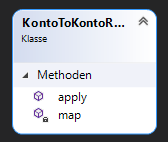
\includegraphics[width=5cm]{KtoKMapperVorher.png}}
    \caption{\label{singletonVorher} Singleton Vorher}
\end{figure}
\begin{figure}[htbp]
    \centering
    \fbox{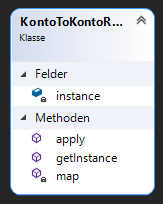
\includegraphics[width=5cm]{KtoKMapperNachher.png}}
    \caption{\label{singletonNachher} Singleton Nachher}
\end{figure}
